% Copyright 2004 by Till Tantau <tantau@users.sourceforge.net>.
%
% In principle, this file can be redistributed and/or modified under
% the terms of the GNU Public License, version 2.
%
% However, this file is supposed to be a template to be modified
% for your own needs. For this reason, if you use this file as a
% template and not specifically distribute it as part of a another
% package/program, I grant the extra permission to freely copy and
% modify this file as you see fit and even to delete this copyright
% notice. 

\documentclass{beamer}

\usepackage{floatrow}%

% There are many different themes available for Beamer. A comprehensive
% list with examples is given here:
% http://deic.uab.es/~iblanes/beamer_gallery/index_by_theme.html
% You can uncomment the themes below if you would like to use a different
% one:
%\usetheme{AnnArbor}
%\usetheme{Antibes}
%\usetheme{Bergen}
%\usetheme{Berkeley}
%\usetheme{Berlin}
%\usetheme{Boadilla}
%\usetheme{boxes}
%\usetheme{CambridgeUS}
%\usetheme{Copenhagen}
%\usetheme{Darmstadt}
%\usetheme{default}
%\usetheme{Frankfurt}
%\usetheme{Goettingen}
%\usetheme{Hannover}
%\usetheme{Ilmenau}
%\usetheme{JuanLesPins}
%\usetheme{Luebeck}
\usetheme{Madrid}
%\usetheme{Malmoe}
%\usetheme{Marburg}
%\usetheme{Montpellier}
%\usetheme{PaloAlto}
%\usetheme{Pittsburgh}
%\usetheme{Rochester}
%\usetheme{Singapore}
%\usetheme{Szeged}
%\usetheme{Warsaw}

\title{How to make a full body 3D scanner}

\author{By: Emile Okada\inst{1}, \\ Supervisors: Carola Schoenlieb\inst{1}, Martin Benning\inst{1}, Matthias Ehrhardt\inst{1}, Veronia Corona\inst{1}}
% - Give the names in the same order as the appear in the paper.
% - Use the \inst{?} command only if the authors have different
%   affiliation.

\institute[University of Cambridge] % (optional, but mostly needed)
{
  \inst{1}%
  DAMTP\\
  University of Cambridge
  }
% - Use the \inst command only if there are several affiliations.
% - Keep it simple, no one is interested in your street address.

\date{Summer Undergraduate Research Talks}
% - Either use conference name or its abbreviation.
% - Not really informative to the audience, more for people (including
%   yourself) who are reading the slides online

\subject{Image Analysis}
% This is only inserted into the PDF information catalog. Can be left
% out. 

% If you have a file called "university-logo-filename.xxx", where xxx
% is a graphic format that can be processed by latex or pdflatex,
% resp., then you can add a logo as follows:

% \pgfdeclareimage[height=0.5cm]{university-logo}{university-logo-filename}
% \logo{\pgfuseimage{university-logo}}

% Delete this, if you do not want the table of contents to pop up at
% the beginning of each subsection:
\AtBeginSubsection[]
{
  \begin{frame}<beamer>{Outline}
    \tableofcontents[currentsection,currentsubsection]
  \end{frame}
}

% Let's get started
\begin{document}

\begin{frame}
  \titlepage
\end{frame}

\begin{frame}{Outline}
  \tableofcontents
  % You might wish to add the option [pausesections]
\end{frame}

% Section and subsections will appear in the presentation overview
% and table of contents.
\section{3D Reconstructions}

\subsection{'Slice-wise' convex volumes}

\begin{frame}{3D Reconstruction}
    \begin{figure}[H]
      \centering
        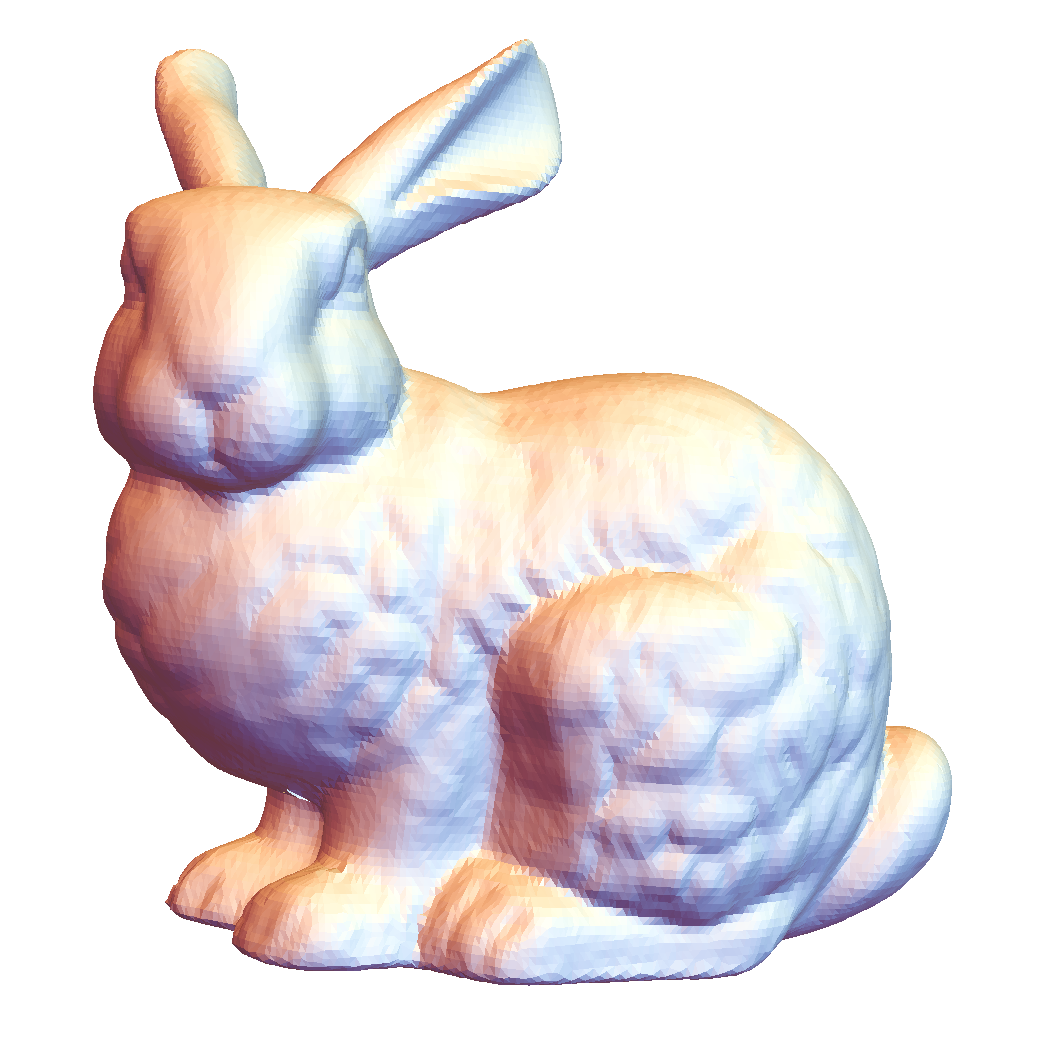
\includegraphics[width=0.5\textwidth]{3D_rabit.png}
      \label{fig:f2}
    \end{figure}
\end{frame}

\begin{frame}{3D Reconstruction}
    \begin{figure}[H]
        \begin{floatrow}
            \ffigbox{
\includegraphics[scale = 0.4]{rabit1.jpg}}{\label{fig:err5}}
            \ffigbox{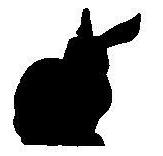
\includegraphics[scale = 0.4]{rabit4.jpg}}{\label{fig:err6}}
        \end{floatrow}
    \end{figure}
    \begin{figure}[H]
        \begin{floatrow}
            \ffigbox{
\includegraphics[scale = 0.4]{rabit7.jpg}}{\label{fig:err7}}
            \ffigbox{
\includegraphics[scale = 0.4]{rabit10.jpg}}{\label{fig:err8}}
        \end{floatrow}
    \end{figure}
\end{frame}

\begin{frame}{3D Reconstruction}
    \begin{figure}[H]
      \centering
        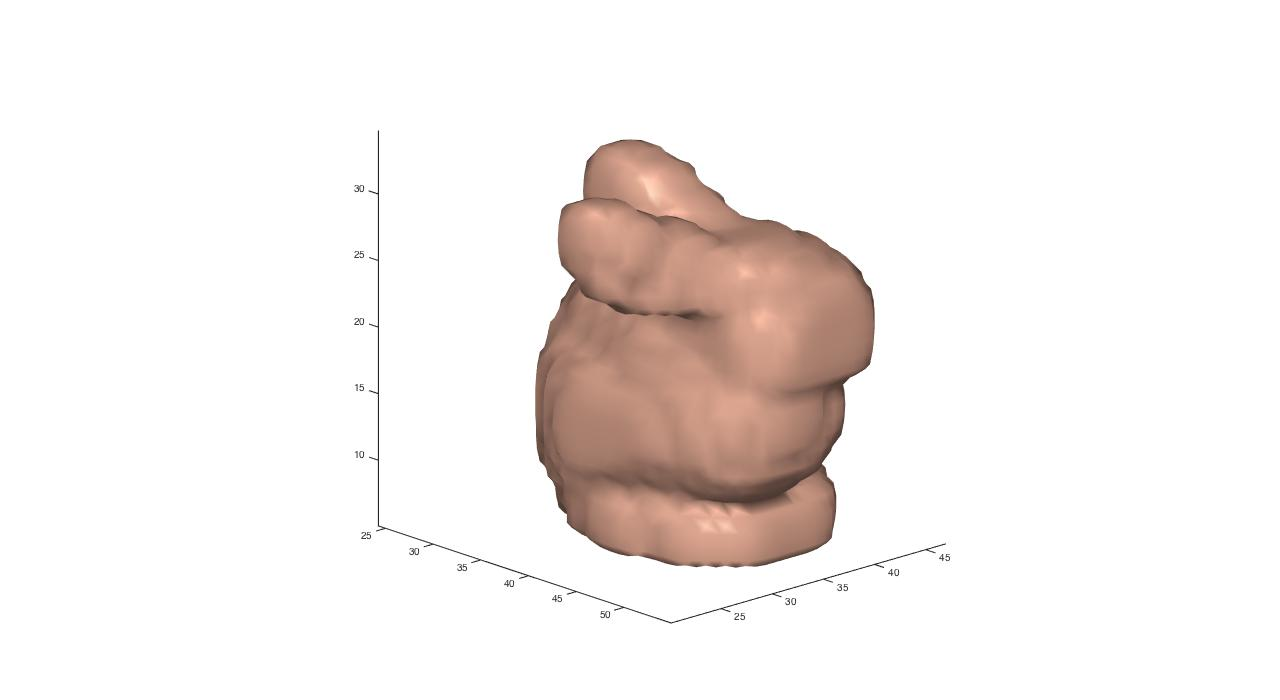
\includegraphics[width=0.8\textwidth]{rabit_surface_1.jpg}
      \label{fig:f2}
    \end{figure}
\end{frame}

\section{Building}
\begin{frame}{Initial design}
    \begin{figure}[H]
      \centering
        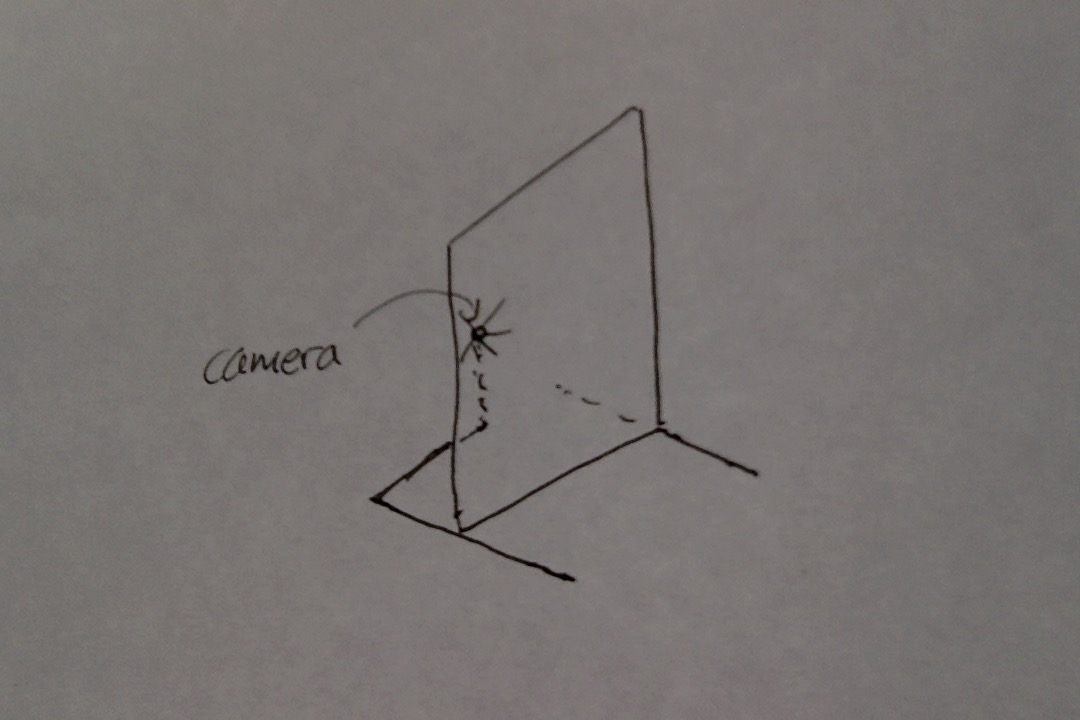
\includegraphics[width=0.8\textwidth]{new_setup.jpg}
      \label{fig:f2}
    \end{figure}
\end{frame}

\begin{frame}{Frame is made}
    \begin{figure}[H]
      \centering
        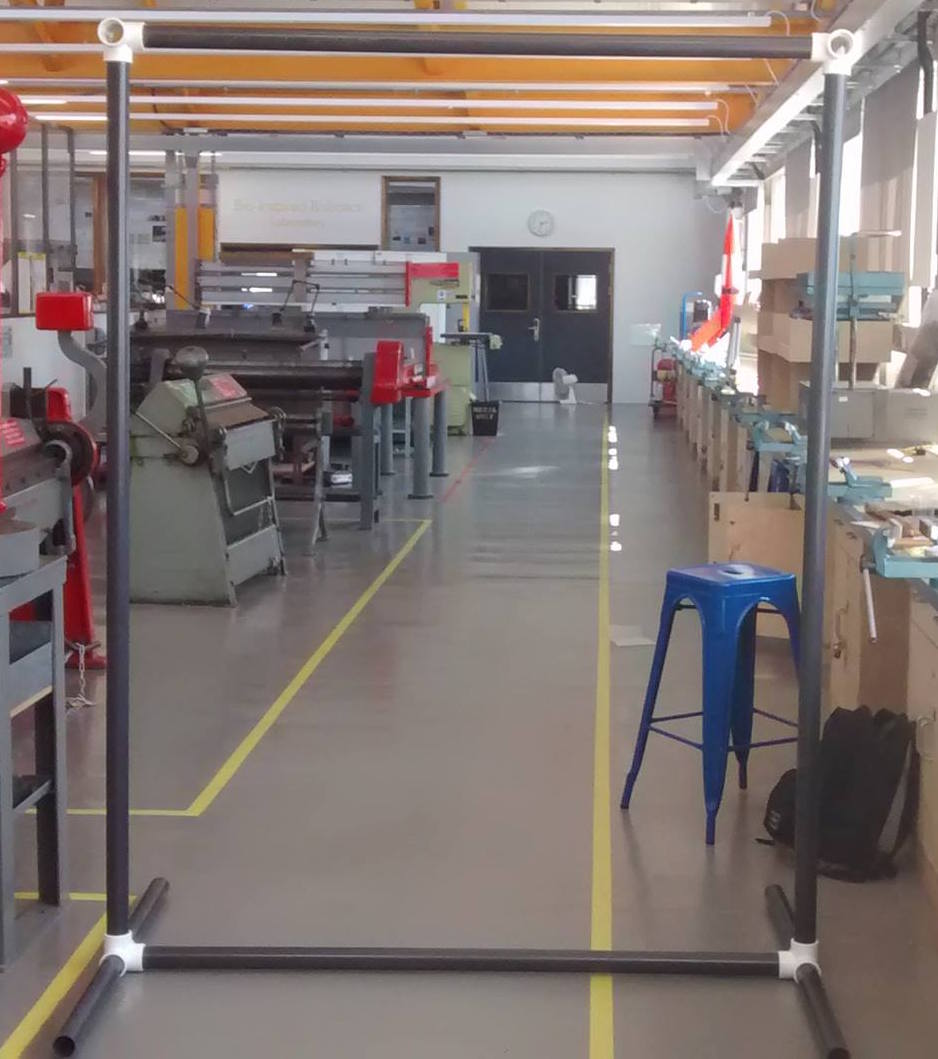
\includegraphics[width=0.5\textwidth]{skeleton.jpg}
      \label{fig:f2}
    \end{figure}
\end{frame}

\begin{frame}{Sewing mathematician in engineering department}
    \begin{figure}[H]
      \centering
        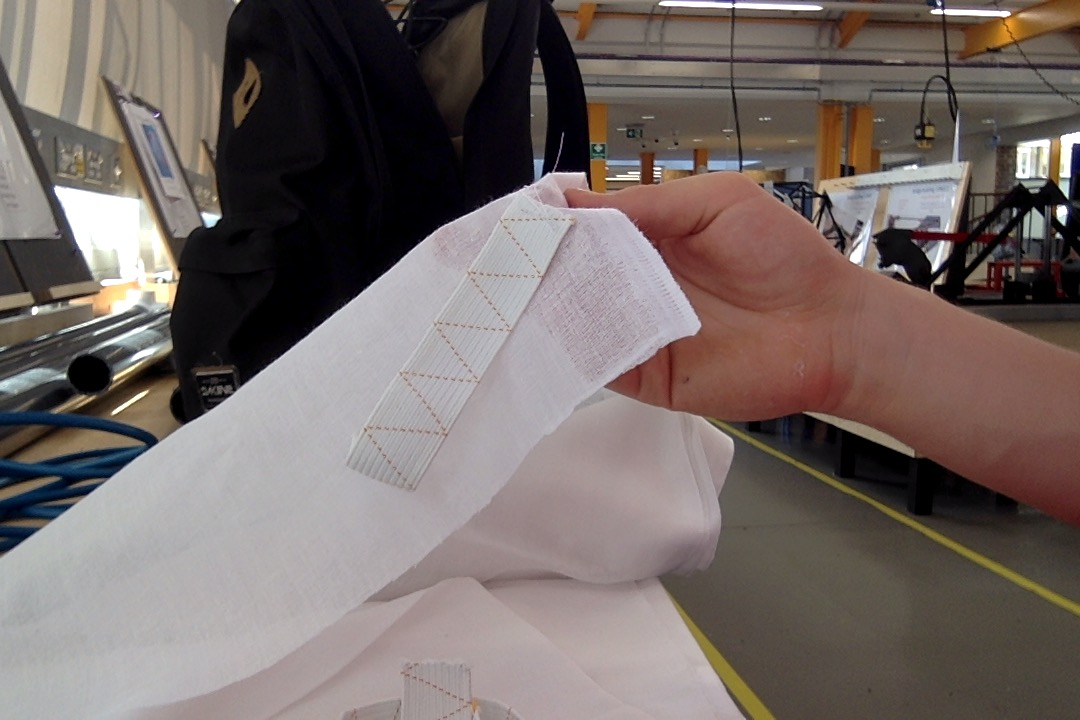
\includegraphics[width=0.8\textwidth]{sewing.jpg}
      \label{fig:f2}
    \end{figure}
\end{frame}

\begin{frame}{Shadow}
    \begin{figure}[H]
      \centering
        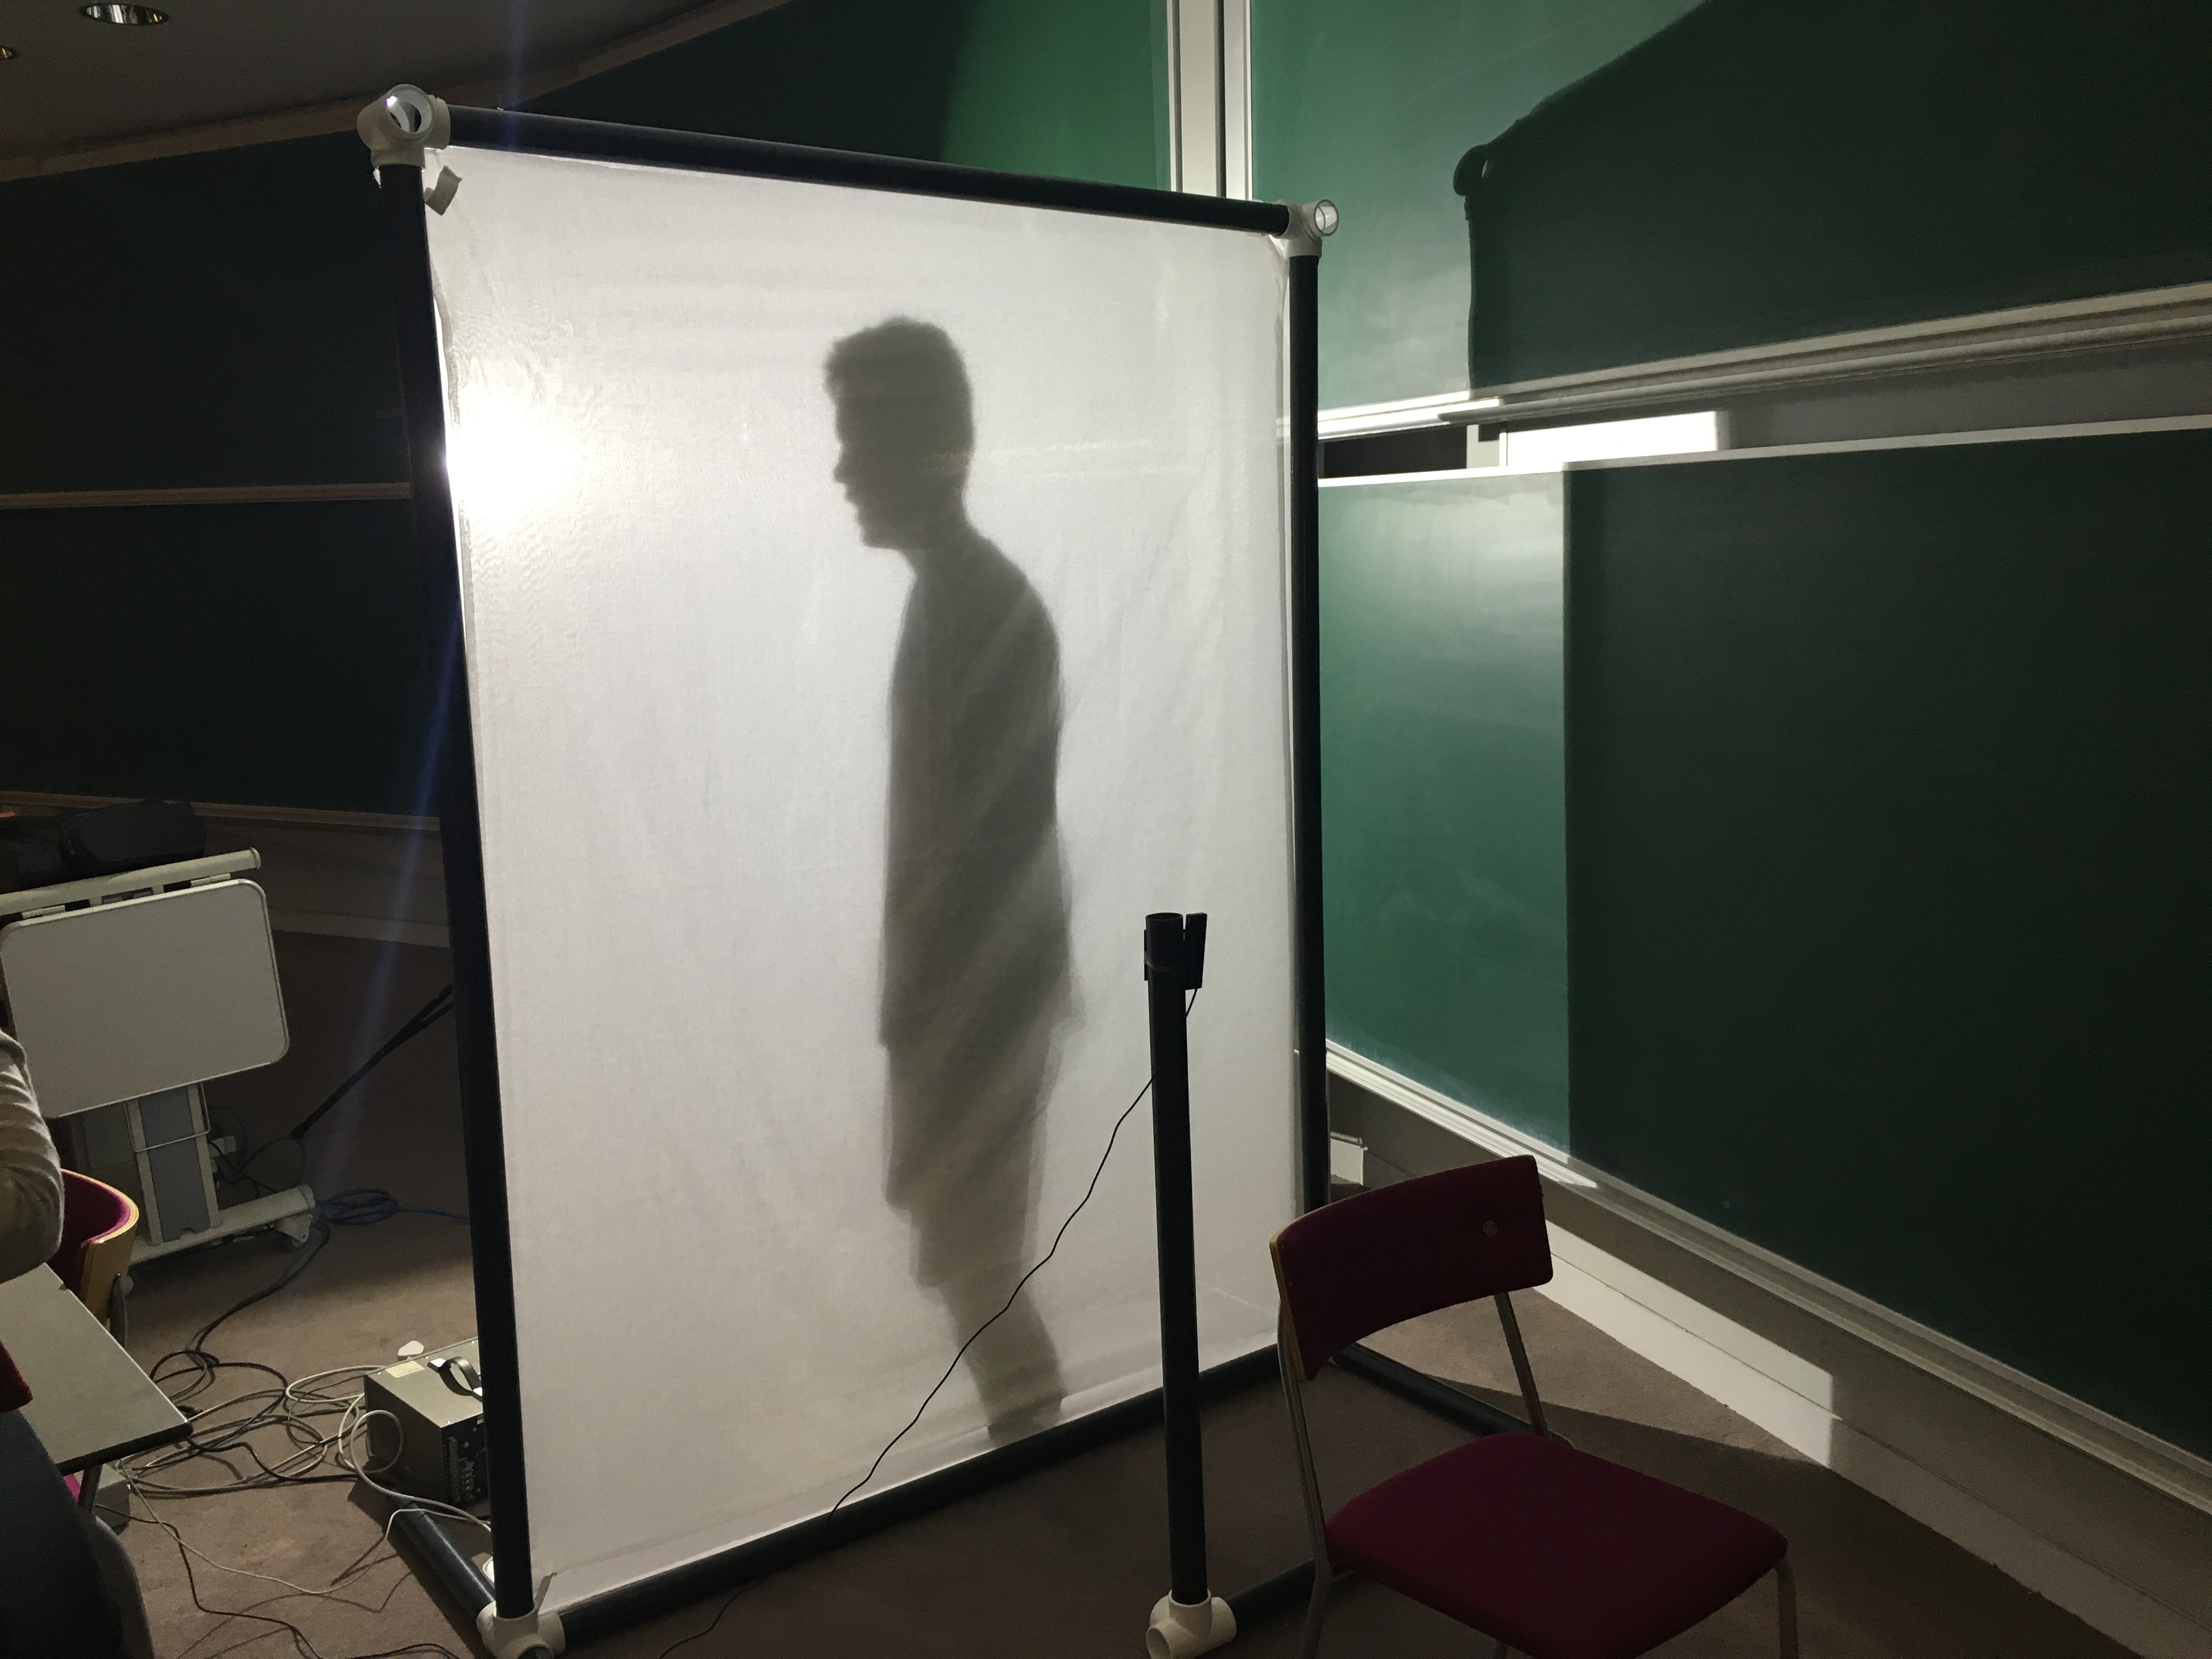
\includegraphics[width=0.8\textwidth]{IMG_5452.jpg}
      \label{fig:f2}
    \end{figure}
\end{frame}

\begin{frame}{3D printing}
    \begin{figure}[H]
      \centering
        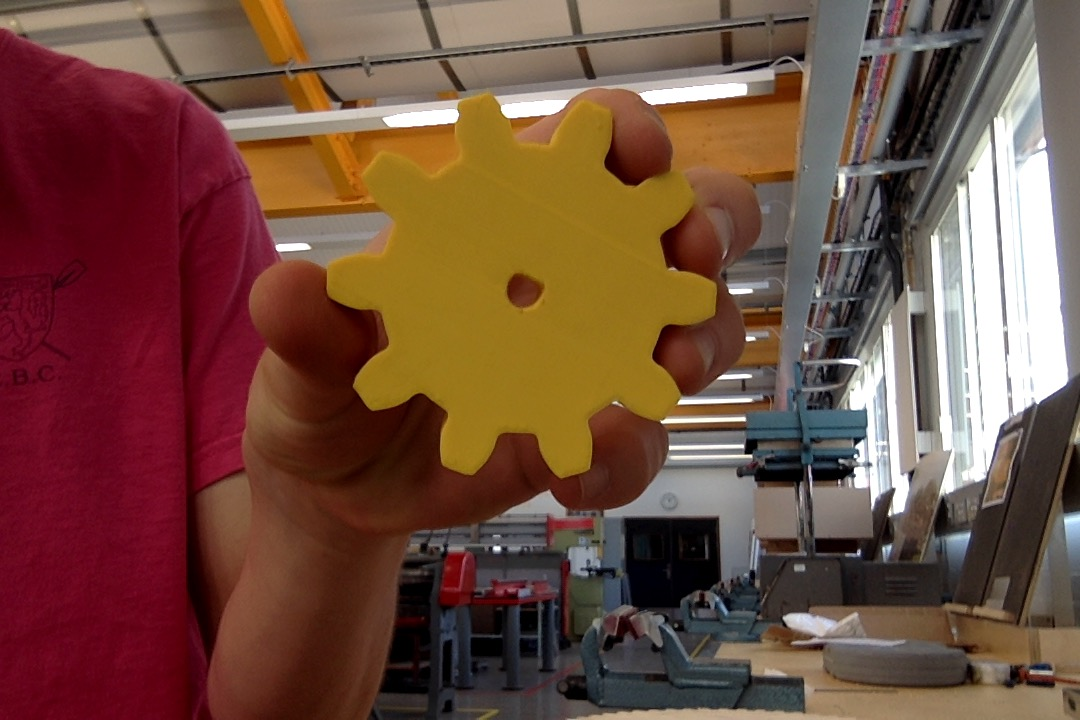
\includegraphics[width=0.8\textwidth]{printed_cog.jpg}
      \label{fig:f2}
    \end{figure}
\end{frame}

\begin{frame}{Making the turntable}
    \begin{figure}[H]
      \centering
        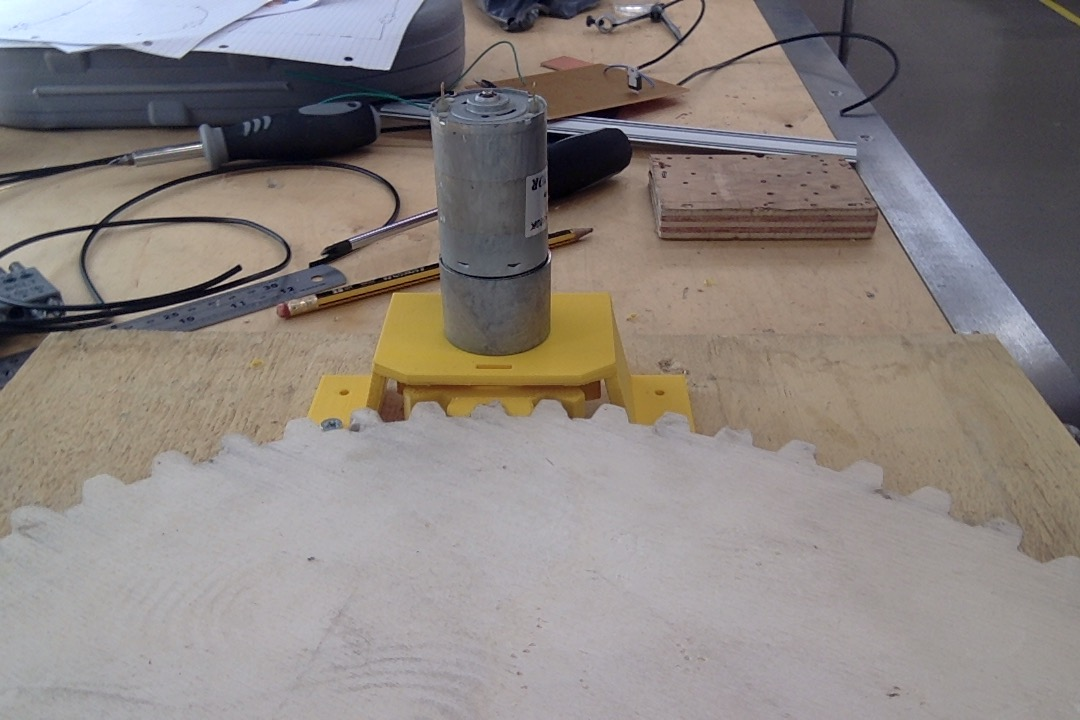
\includegraphics[width=0.8\textwidth]{mounted_motor.jpg}
      \label{fig:f2}
    \end{figure}
\end{frame}

\begin{frame}{Making the turntable}
    \begin{figure}[H]
      \centering
        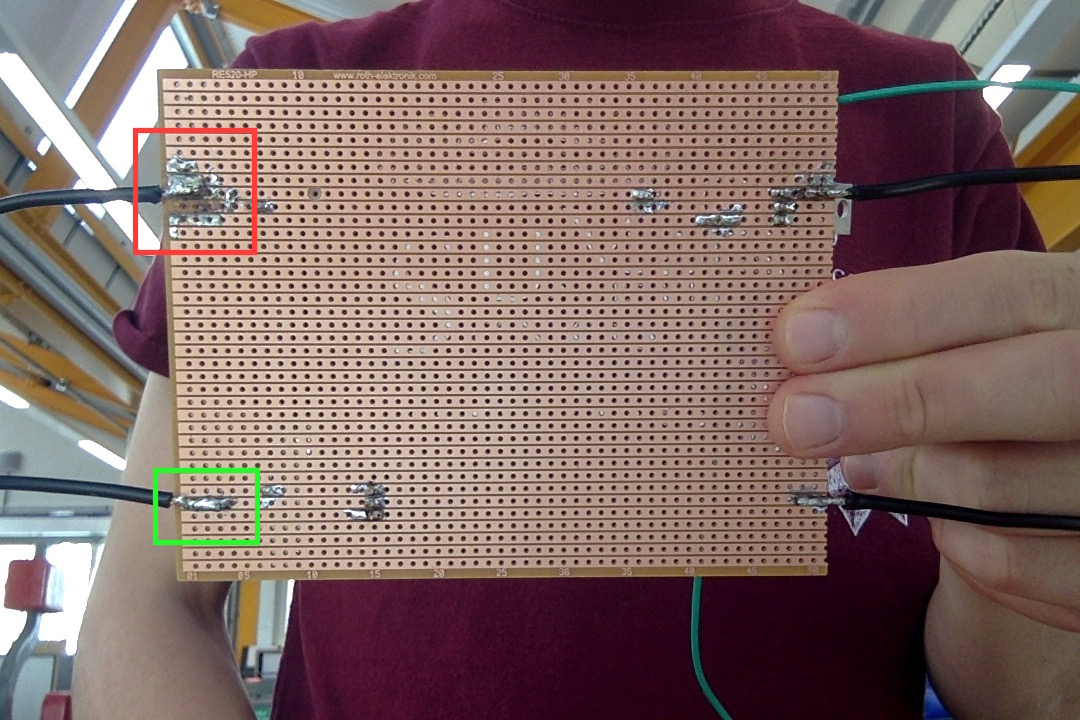
\includegraphics[width=0.8\textwidth]{circuit_1_red.jpg}
      \label{fig:f2}
    \end{figure}
\end{frame}

\begin{frame}{Turntable}
    \begin{figure}[H]
      \centering
        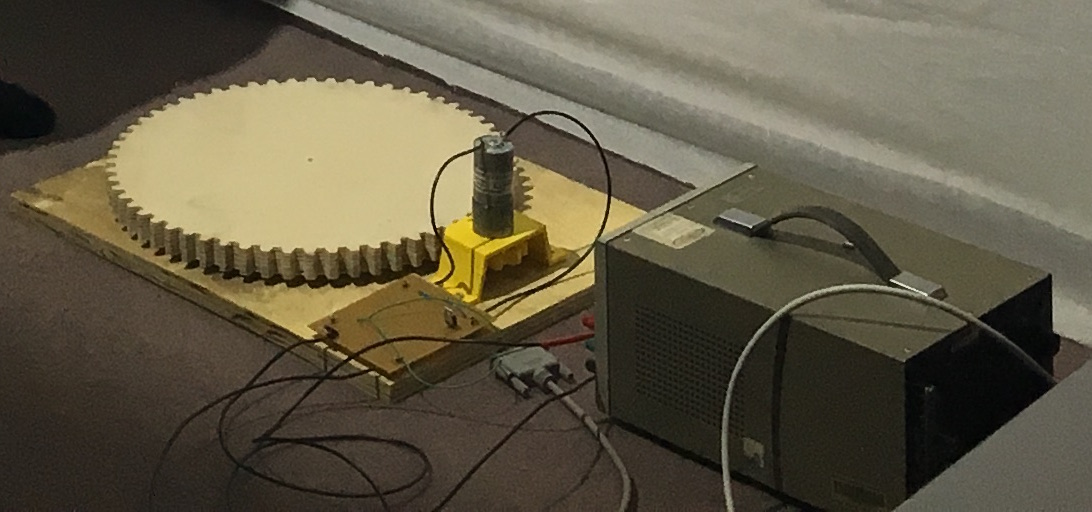
\includegraphics[width=0.8\textwidth]{assembly.jpg}
      \label{fig:f2}
    \end{figure}
\end{frame}

\begin{frame}{Whole set-up}
    \begin{figure}[H]
      \centering
        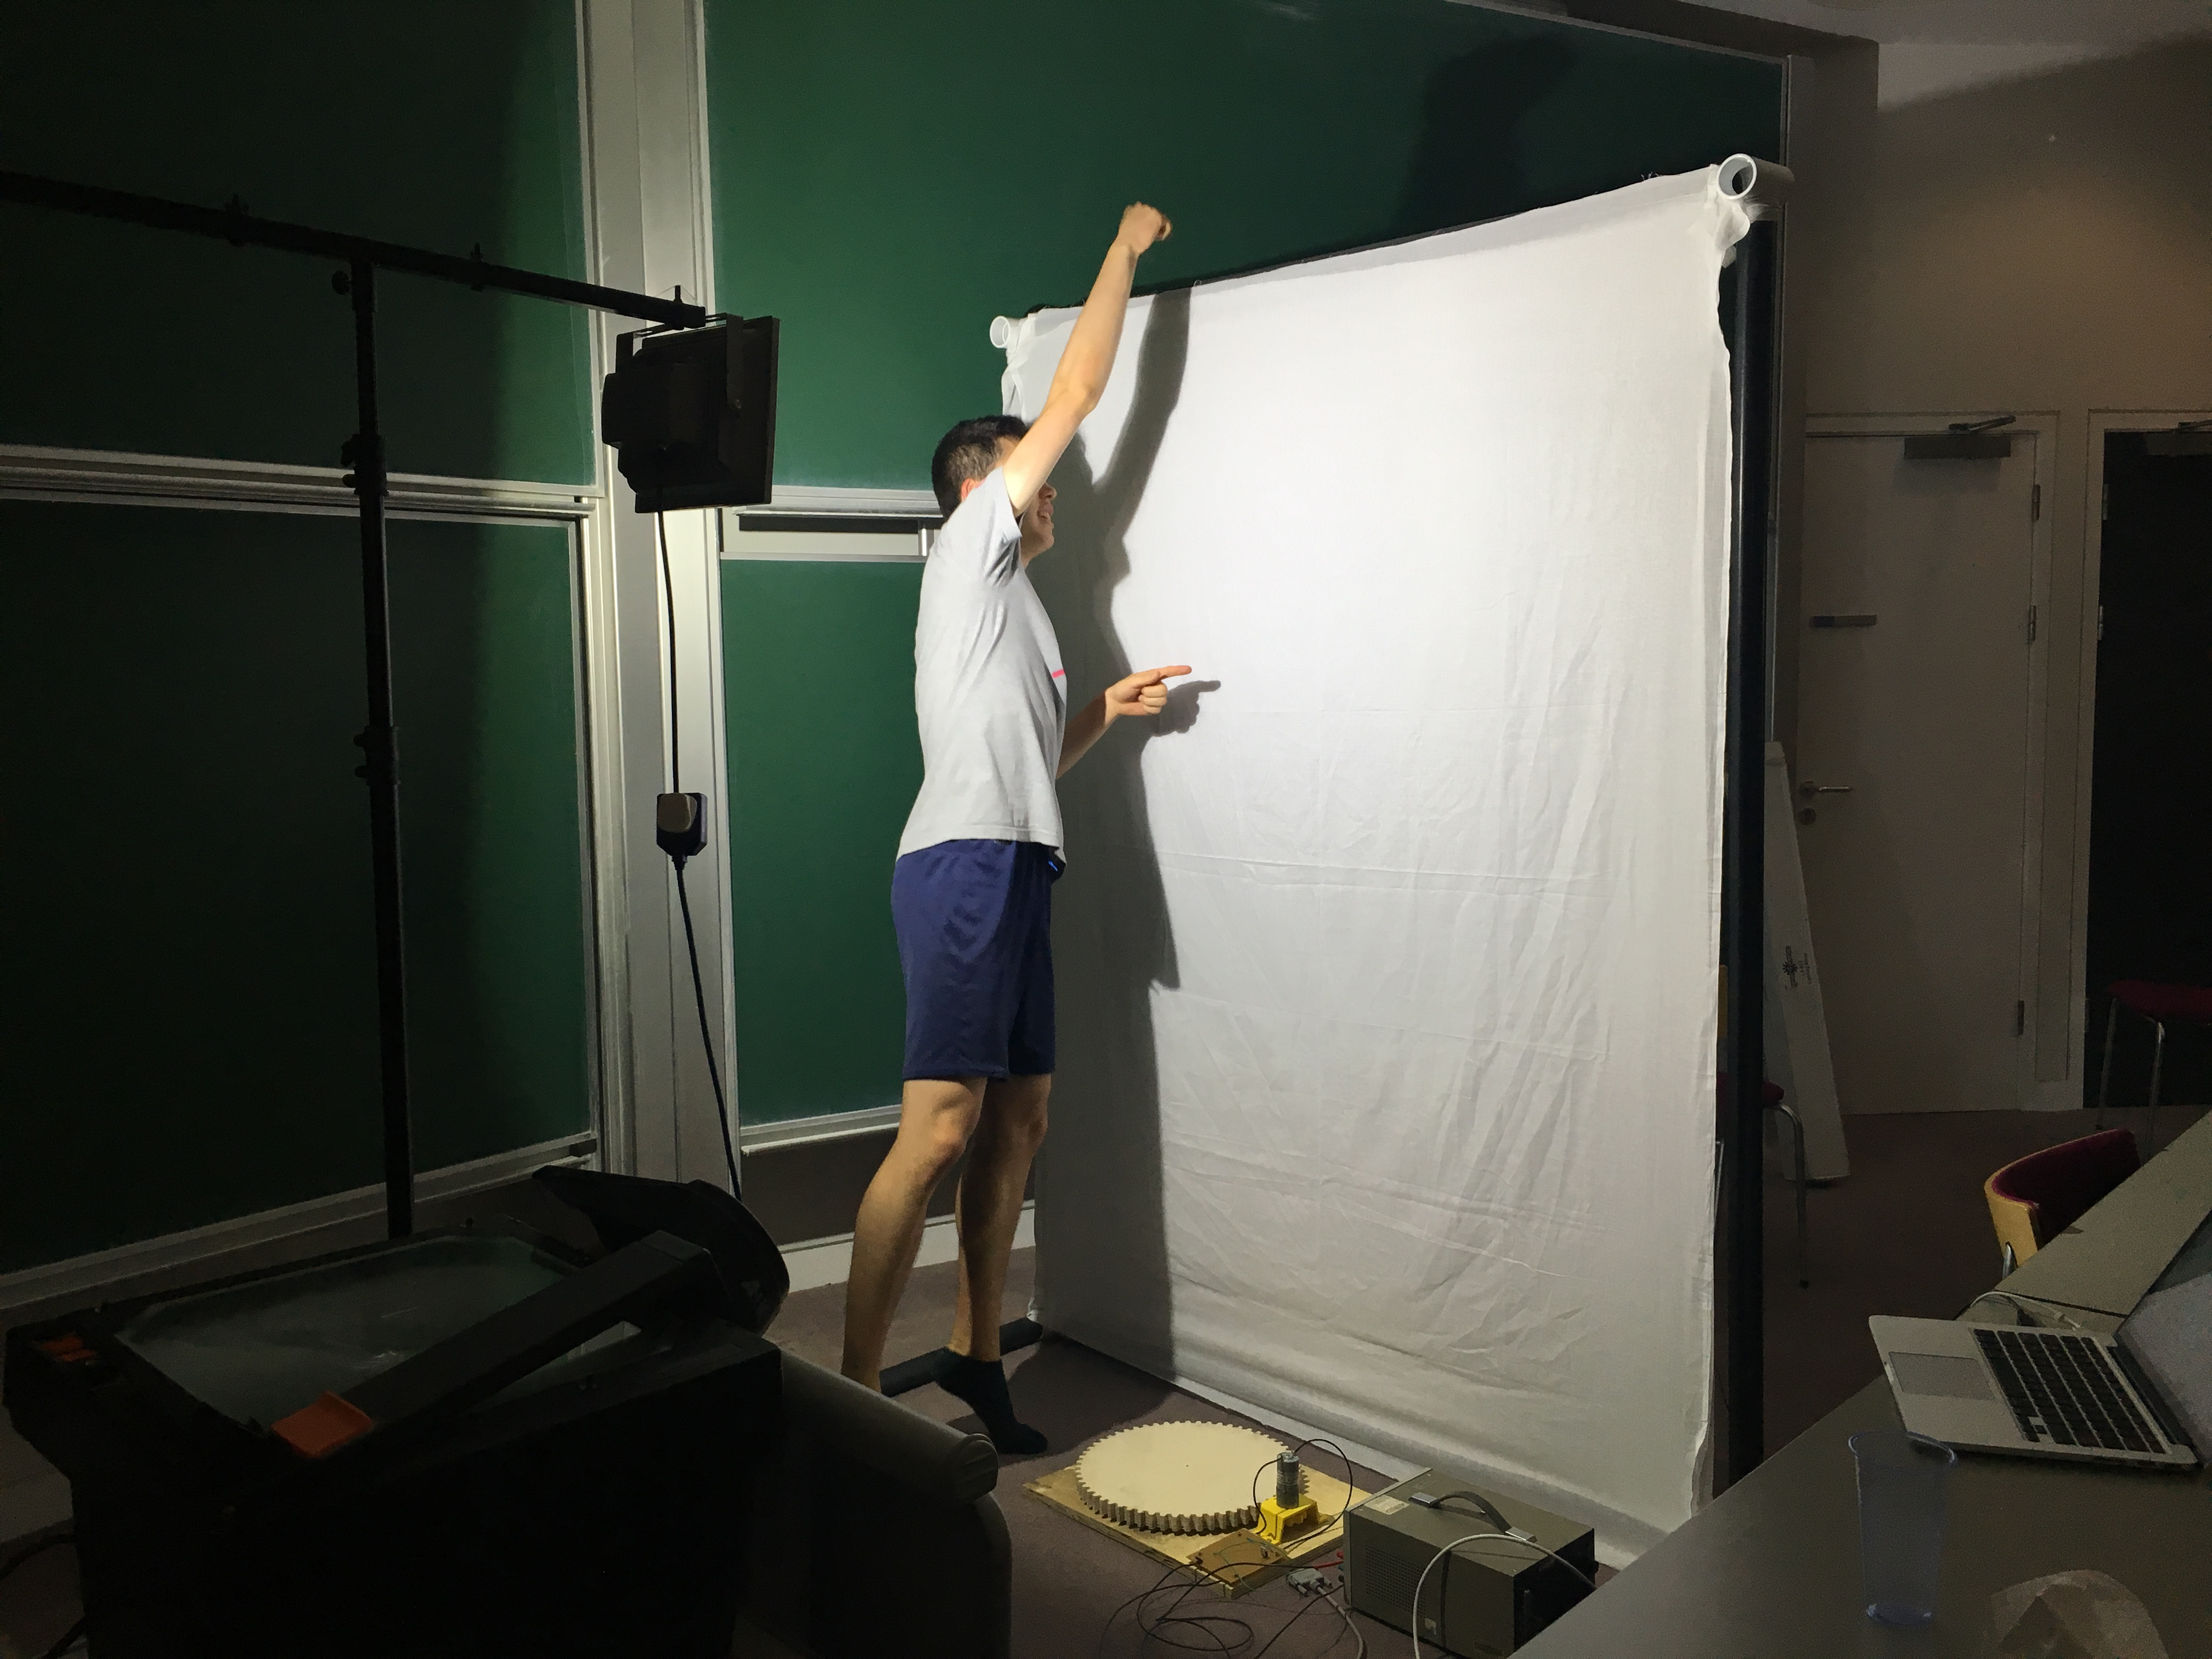
\includegraphics[width=0.8\textwidth]{IMG_5444.jpg}
      \label{fig:f2}
    \end{figure}
\end{frame}

\begin{frame}{Reconstruction}
    \begin{figure}[H]
      \centering
        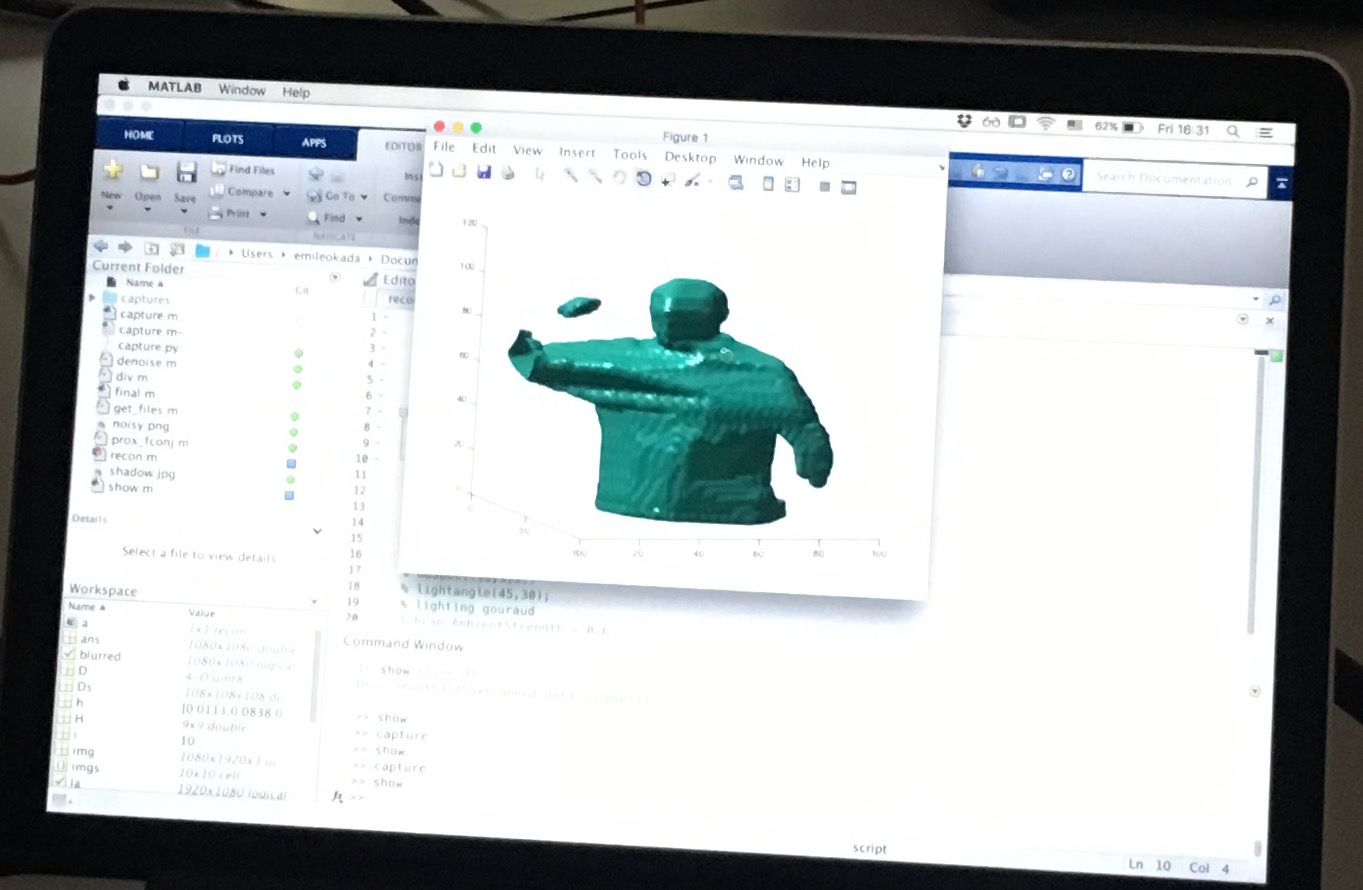
\includegraphics[width=0.8\textwidth]{martin_recon.jpg}
      \label{fig:f2}
    \end{figure}
\end{frame}

\section{TV Denoising}

\begin{frame}{TV Denoising}
    \begin{equation}
        \min_{u}\int_{\Omega}|Du|+\frac12\lambda \|u-f\|_2^2 \nonumber
    \end{equation}
\end{frame}

\end{document}


